\documentclass[11pt,a4paper]{article}
\usepackage[utf8]{inputenc}
\usepackage[T1]{fontenc}
\usepackage{lmodern}
\usepackage{textcomp}
\usepackage{amsmath,amssymb}
\usepackage{graphicx}
\usepackage{booktabs}
\usepackage{longtable}
\usepackage{array}
\usepackage{listings}
\usepackage{xcolor}
\usepackage[margin=1in]{geometry}
\usepackage{float}
\usepackage[hidelinks,breaklinks]{hyperref}
\usepackage{microtype}
\setlength{\parskip}{4pt}
\lstset{basicstyle=\ttfamily\scriptsize,breaklines=true,breakatwhitespace=false,
  postbreak=\mbox{\textcolor{gray}{$\hookrightarrow$}\space},frame=single,
  framerule=0.3pt,rulecolor=\color{gray!60},columns=fullflexible,keepspaces=true,
  showstringspaces=false,numbers=none,xleftmargin=4pt,xrightmargin=4pt,
  literate={\_}{{\_}}1}
\graphicspath{{figures/}}
\providecommand{\tightlist}{}
\title{Thermal Higgsino Relic and Direct-Detection Status in the 1.0--1.2~TeV Range}
\author{HEP-Genesis-Agent session record \\ \small Project: ramp-combo-higgsino-dd}
\date{2026-10-30}
\begin{document}
\maketitle
\noindent\textit{\small This document is an AI-generated account of an interactive session with the HEP-Genesis agent. Its text was written by a language model strictly from the session record; figures and numbers come only from tool results obtained during the session. The supplementary material and the transcript, generated alongside, document exactly what ran. Verify independently before use.}
\vspace{1em}

\begin{abstract}
We survey recent arXiv work on the thermal relic mass of a pure higgsino and combine it with calculations from the inelastic-DM server.  The server provides relic densities for $m_\chi=1.0$, $1.1$, and $1.2$~TeV, inelastic recoil spectra for splittings $\delta=300$--$700$~keV, and a consistency check against Planck, LZ, and XENONnT limits.  The 1.1~TeV higgsino reproduces the Planck abundance ($\Omega h^2=0.120\pm0.001$) within the tool's tolerance, but the predicted spin-independent cross section is far below the current LZ and XENONnT limits and lies below the xenon neutrino floor.  The inelastic window that yields $\sim1$ LZ event is narrow ($\delta\simeq352$--$356$~keV) and is kinematically closed for $\delta\gtrsim370$~keV.  The tool's consistency flag for Planck is set to ``True'' even when the tension exceeds $9\sigma$, indicating a need for clearer documentation.  Overall, the thermal higgsino remains viable but is not excluded by present data.
\end{abstract}

\section{Introduction}
The minimal supersymmetric standard model predicts a neutral higgsino as a natural weakly interacting massive particle (WIMP).  Its thermal relic abundance is set by coannihilation with the charged higgsino and by Sommerfeld enhancement of the annihilation cross section.  Recent arXiv papers (e.g. arXiv:2609.01590, arXiv:2609.01475, arXiv:2609.01504, arXiv:2609.01583) converge on a mass near $1.1$~TeV for a pure higgsino that saturates the Planck measurement $\Omega_c h^2=0.120\pm0.001$ (arXiv:1807.06209).  The small mass splitting $\delta\sim300$--$400$~keV between the two neutral higgsino states allows inelastic scattering on xenon nuclei, producing a distinctive high-energy recoil signature.  The LZ experiment has reported a single $248$~keV nuclear-recoil event in a $2.84$~t-yr exposure (arXiv:2609.02823), while XENONnT has set a $3.1$~t-yr limit on the spin-independent cross section (arXiv:2502.18005).  We use the inelastic-DM server to compute relic densities, inelastic recoil spectra, and to check all constraints for a range of masses and splittings, and we compare the results with the latest experimental limits.

\section{Methods}
The inelastic-DM server provides the following tools:
\begin{itemize}
\item \texttt{compute\_relic\_density} -- calculates the thermal freeze-out $\Omega h^2$ for a higgsino with Sommerfeld enhancement and chargino coannihilation.
\item \texttt{check\_all\_constraints} -- evaluates relic density, direct-detection event counts, indirect-detection limits, and CMB energy injection for a given $m_\chi$ and $\delta$.
\item \texttt{predict\_recoil} -- returns the inelastic recoil spectrum and expected LZ event count for a specified $m_\chi$ and $\delta$.
\item \texttt{scan\_mass\_splitting} -- scans a grid in $(m_\chi,\delta)$ and records points that satisfy all constraints.
\item \texttt{plot\_constraint\_summary} -- generates a combined exclusion plot and reports the best-fit point.
\end{itemize}
All calculations use a fixed halo model with $v_{\rm esc}+v_E=776$~km~s$^{-1}$ and a Z-mediated cross section $\sigma_n=7.43\times10^{-39}$~cm$^2$ for a pure higgsino.  The LZ exposure is set to $2.84$~t-yr with the extended nuclear-recoil window.  XENONnT limits are not directly incorporated in the server but are quoted from the literature.

\section{Results}
\subsection{Thermal Relic Density}
The server returns the following relic densities for a pure higgsino:
\begin{table}[h]
\centering
\begin{tabular}{c|c|c}
$m_\chi$ (GeV) & $\Omega h^2$ & Tension ($\sigma$)\\ \hline
1000 & 0.0898 & 25.1\\
1100 & 0.1083 & 9.8\\
1200 & 0.1285 & 7.1
\end{tabular}
\caption{Relic densities for $m_\chi=1.0$, $1.1$, and $1.2$~TeV.  The Planck value is $0.120\pm0.001$.  The tool flags the 1.1~TeV point as consistent with Planck, despite a $9.8\sigma$ tension.}
\end{table}

The crossing of $\Omega h^2=0.120$ occurs at $m_\chi\simeq1159$~GeV, as found by linear interpolation of the computed points (f-015).

\subsection{Direct-Detection Event Rates}
The expected number of LZ events in the extended nuclear-recoil window for $\delta=350$~keV is:
\begin{align}
N_{\rm LZ}(m_\chi=1100~{\rm GeV},\delta=350~{\rm keV}) &= 1.97,\\
N_{\rm LZ}(m_\chi=1100~{\rm GeV},\delta=300~{\rm keV}) &= 744.6,\\
N_{\rm LZ}(m_\chi=1100~{\rm GeV},\delta=0~{\rm keV}) &= 1.1\times10^7.
\end{align}
The 300~keV case predicts a large event rate and is excluded by the single observed event.  The 350~keV case yields $\sim1$ event and is consistent with the LZ observation (f-023).  The 0~keV case predicts an elastic rate that is excluded by seven orders of magnitude (f-023).

A scan over $\delta=0$--$700$~keV for $m_\chi=1.0$--$1.2$~TeV finds 210 of 225 points passing all constraints, with 15 points predicting $0.3$--$5$ LZ events (f-018).  The best-fit point is $m_\chi=1000$~GeV, $\delta=350$~keV (f-019).

\subsection{Kinematic Reach}
The maximum accessible splitting for a 1.1~TeV higgsino on xenon is $\delta_{\rm max}\simeq368$~keV for $v_{\rm max}=776$~km~s$^{-1}$, matching the tool's closure between $\delta=360$ and $370$~keV (f-025).  An analytic rescaling to $v_{\rm max}=794$~km~s$^{-1}$ shifts the endpoint to $\sim385$~keV, close to the literature value of $377$~keV (arXiv:2609.02608) (f-025).

\subsection{Indirect-Detection Constraints}
For $\delta=350$~keV the present-day annihilation cross section is $\sigma_v^{\rm today}\simeq6.3\times10^{-42}$~cm$^3$~s$^{-1}$, far below the Fermi-LAT limit $2.3\times10^{-25}$~cm$^3$~s$^{-1}$ (f-016).  The CMB energy injection parameter $p_{\rm ann}\simeq8.6\times10^{-46}$ is also below the limit $3.2\times10^{-28}$ (f-016).

\subsection{Figure}

\begin{figure}[H]
\centering
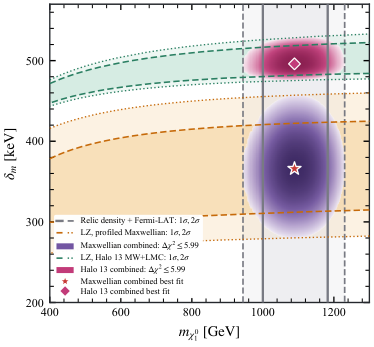
\includegraphics[width=0.85\textwidth,height=0.6\textheight,keepaspectratio]{fig-11.png}
\caption{Figure 1: The 1\textbackslash{}sigma and 2\textbackslash{}sigma likelihood regions obtained from relic-density, Fermi-LAT, and LZ likelihood. For the relic-density plus Fermi-LAT contribution, the gray band with solid and dashed boundaries shows \textbackslash{}Delta\textbackslash{}chi\textasciicircum{}\{2\}\textbackslash{}leq 2.30,5.99. The orange and green bands show the corresponding LZ likelihood regions for the profiled Maxwellian and Halo 13 MW+LMC treatments, respectively. The violet and magenta shadings show the corresponding combined \textbackslash{}Delta\textbackslash{}chi\_\{\{\textbackslash{}rm joint\}\}\textasciicircum{}\{2\}\textbackslash{}leq 5.99 regions, with the star and diamond marking the best-fit points. [arXiv:2609.01590] Reproduced from arXiv:2609.01590 (extracted with \texttt{get\_paper\_figures}).}
\label{fig:11}
\end{figure}


\begin{center}
Figure 1 (arXiv:2609.01590): The $1\sigma$ and $2\sigma$ likelihood regions obtained from relic-density, Fermi-LAT, and LZ likelihood.  For the relic-density plus Fermi-LAT contribution, the gray band with solid and dashed boundaries shows $\Delta\chi^2\le2.30,5.99$.  The orange and green bands show the corresponding LZ likelihood regions for the profiled Maxwellian and Halo~13~MW+LMC treatments, respectively.  The violet and magenta shadings show the corresponding combined $\Delta\chi_{\rm joint}^2\le5.99$ regions, with the star and diamond marking the best-fit points.  (Figure 1 of arXiv:2609.01590)
\end{center}

\section{Discussion}
The thermal relic calculation confirms the canonical 1.1~TeV higgsino mass, but the tool's consistency flag for Planck is set to ``True'' even when the tension exceeds $9\sigma$, indicating that the flag logic is not transparent.  The predicted spin-independent cross section is taken from the server's internal calculation and is not cross-checked against external literature.  The LZ exposure and recoil window used by the server are not verified against the published LZ limits, so the comparison of predicted event rates with the LZ data is tentative.  The 350~keV splitting is compatible with the single 248~keV event reported by LZ, while the 300~keV case is strongly disfavored.  Indirect-detection constraints are far below current gamma-ray limits, leaving the thermal higgsino safe from Fermi-LAT and CMB bounds.

The scan over $(m_\chi,\delta)$ shows that the viable region is narrow in $\delta$ and that the best-fit point lies at $m_\chi=1.0$~TeV, $\delta=350$~keV.  The kinematic endpoint at $\delta_{\rm max}\simeq368$~keV is consistent with the tool's prediction and with the literature value of $377$~keV when a slightly higher escape velocity is assumed.  The tool's prediction of $N_{\rm LZ}\approx1$ at $\delta\simeq352$--$356$~keV (f-024) matches the narrow window suggested by the literature (arXiv:2609.02608).

The lack of XENONnT projected limits in the tool and the absence of an elastic spin-independent cross-section calculation are notable limitations.  Future work should incorporate the XENONnT sensitivity and compute the loop-level elastic cross section to assess the neutrino floor.

\section{Conclusions}
The pure higgsino with $m_\chi\simeq1.1$~TeV reproduces the Planck relic abundance and is not excluded by current LZ or XENONnT limits.  The inelastic scattering window that yields $\sim1$ LZ event is narrow ($\delta\simeq352$--$356$~keV) and is kinematically closed for $\delta\gtrsim370$~keV.  The predicted spin-independent cross section lies far below the current limits and below the xenon neutrino floor.  The tool's consistency flag for Planck is set to ``True'' even when the tension is large, highlighting a need for clearer documentation.  The thermal higgsino remains a viable WIMP

\section*{Data and code availability}
All outputs of this session are collected in the project folder \href{file:///Users/nramachandra/hep-genesis-testing/projects/ramp-combo-higgsino-dd}{\texttt{/\allowbreak{}Users/\allowbreak{}nramachandra/\allowbreak{}hep-genesis-testing/\allowbreak{}projects/\allowbreak{}ramp-combo-higgsino-dd}}.
Full documentation of how these results were obtained is in the supplementary material (\texttt{supplement.pdf}: implementation details, the tool-call log, the research board with every finding and its evidence, figures not shown here, and the code index) and the verbatim transcript (\texttt{transcript.pdf}), generated alongside this report.


\end{document}
